%%%%%%%%%%%%%%%%%%%%%%%%%%%%%%%%%%%%%%%%%%%%%%%%%%%%%%%%
%%%%                                              %%%%%%
%%%%  Author: Peter Wilson                        %%%%%%
%%%%                                              %%%%%%
%%%%  Shell applications                       %%%%%%
%%%%                                              %%%%%%
%%%%%%%%%%%%%%%%%%%%%%%%%%%%%%%%%%%%%%%%%%%%%%%%%%%%%%%%


%fref generates automatically the respective abreviation/word in the text for the reference. You just have to define a label starting with the respective keyword.
%english: chap, sec, fig, eq, app
%deutsch: chap/kap, abs, abb, gl, anh
%see http://ctan.space-pro.be/tex-archive/macros/latex/contrib/fancyref/fancyref.pdf for more \section

%\onehalfspacing
%\setlength{\belowcaptionskip}{-17pt}

\chapter{Application of shell finite elements}
\label{chap:chapter_application}

\renewcommand{\Thema}{Application of shell finite elements}

\lettrine[lines=2]{W}{ith} the elements formulation, background and validation complete, some examples of their application are now considered. An emphasis is placed on the relative strengths and weaknesses of each element and the effect of their enhancements by considering six elements for each analysis: ANDES-DKQ, Basic-DKQ, Kratos-Q4, DSG, Basic-T3, Kratos-T3.

\section{Euler buckling of CHS column}
\label{applications: Euler buckling of CHS column}
The first application considered is the classic Euler buckling of a slender beam $L=3m$ with a Circular Hollow Section (CHS) of $D = 300mm, t = 5mm$ subject to an axial compressive load $P$. Young's modulus and Poisson's ratio are $E = 206.9GPa$ and $\nu = 0.0$ respectively. The following diagram highlights the system setup with the end restraints imposed corresponding to an Euler case 4 buckling regime. 

\begin{figure}[H]
	\centering
	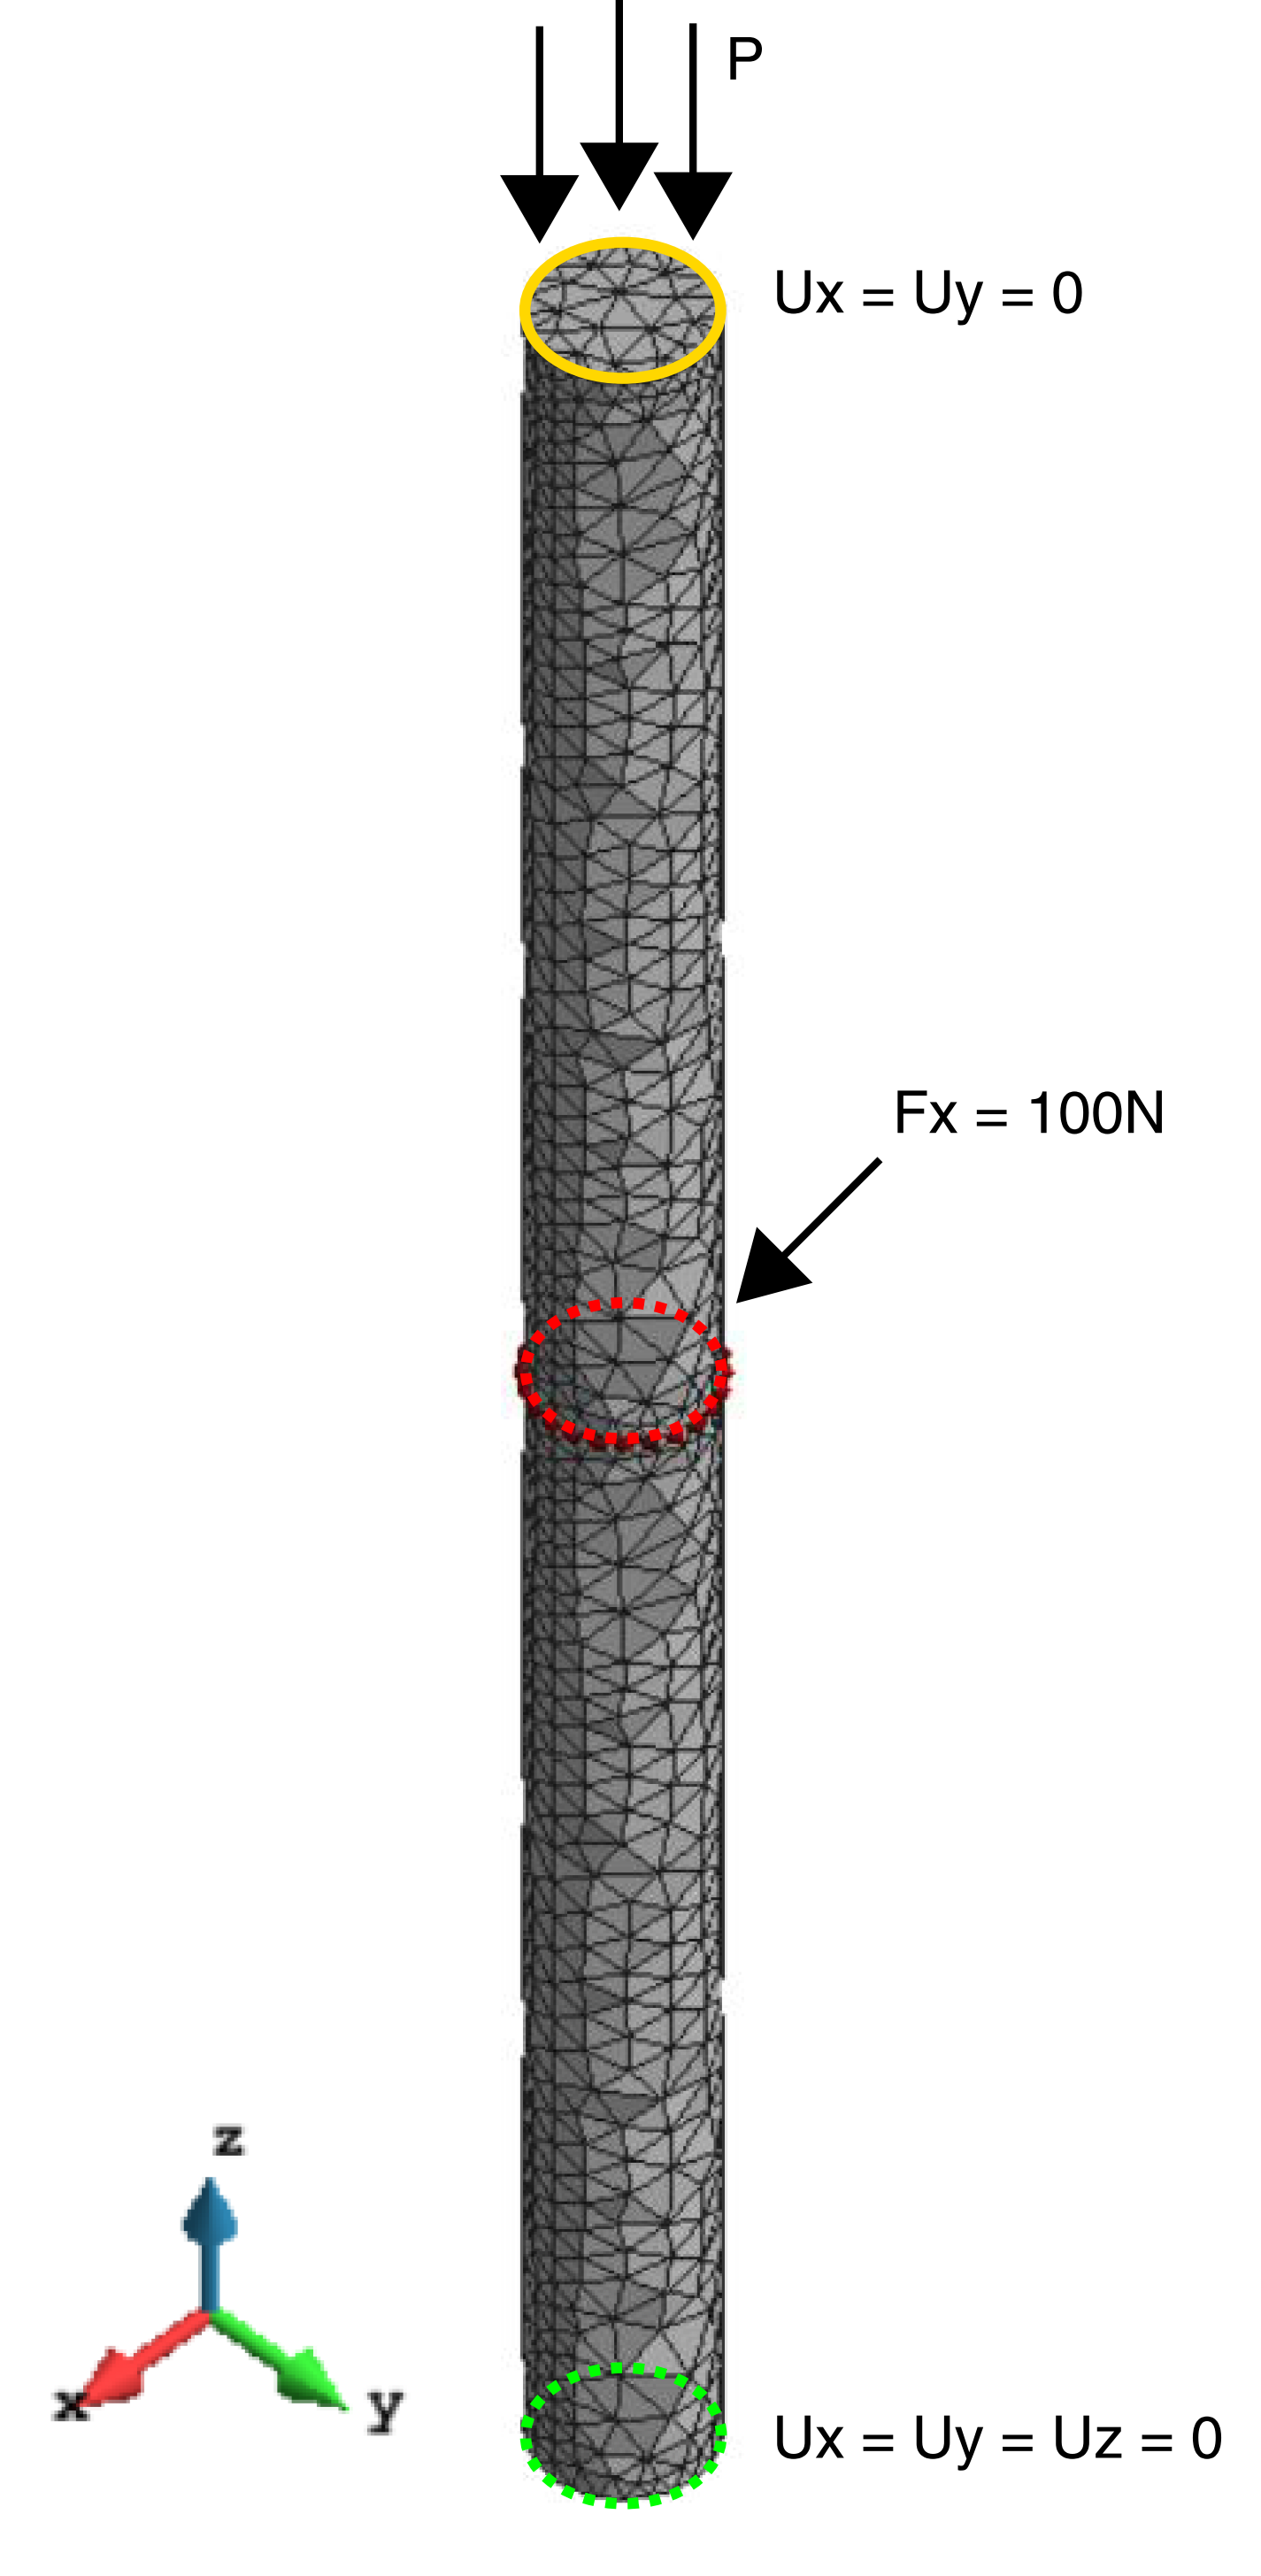
\includegraphics[height=12cm]{images/chs_buckling_setup}
	\caption{CHS buckling setup}
	\label{fig:chsbucklingsetup}
\end{figure}

A full derivation of the Euler case 4 buckling load using beam theory is presented in Appendix \ref{app:Derivation of Euler buckling load} in which the critical load corresponding to the first eigenvalue is:

\begin{equation} 
P_{crit} = \frac{4\pi^2 EI}{L^2} = 13, 222 kN
\label{eqchs_1}
\end{equation}

Due to the unpredictable nature of solving bifurcation problems with FEM a small side load $F_x = 0.1 kN$ is added to a horizontal ring of nodes at the beam's mid-span to encourage switching to the secondary equilibrium path defined by buckling in the XZ plane. Without this side load, or some other reliable source of imperfection, it is possible that the FE model would continue along the primary equilibrium path after the first critical point, instead of switching to a secondary path of buckling. Although the unstructured meshes used may provide enough asymmetry to act as a buckling catalyst, the severity of the imbalance would no doubt change from triangular to quadrilateral unstructured meshes, which may affect the results. Conversely, it's supposed that the applied small lateral load provides a consistent source of imperfection  of greater magnitude than the underlying mesh imbalances, thereby allowing an apples to apples comparison between triangular and quadrilateral meshes.

The first set of results for the analysis highlighting axial displacement (of the top end) vs axial load $P$ is presented below, with circles indicating the onset of instability. Post-critical behaviour has been omitted for clarity.

\begin{figure}[H]
	\centering
	\def\svgwidth{\columnwidth}
	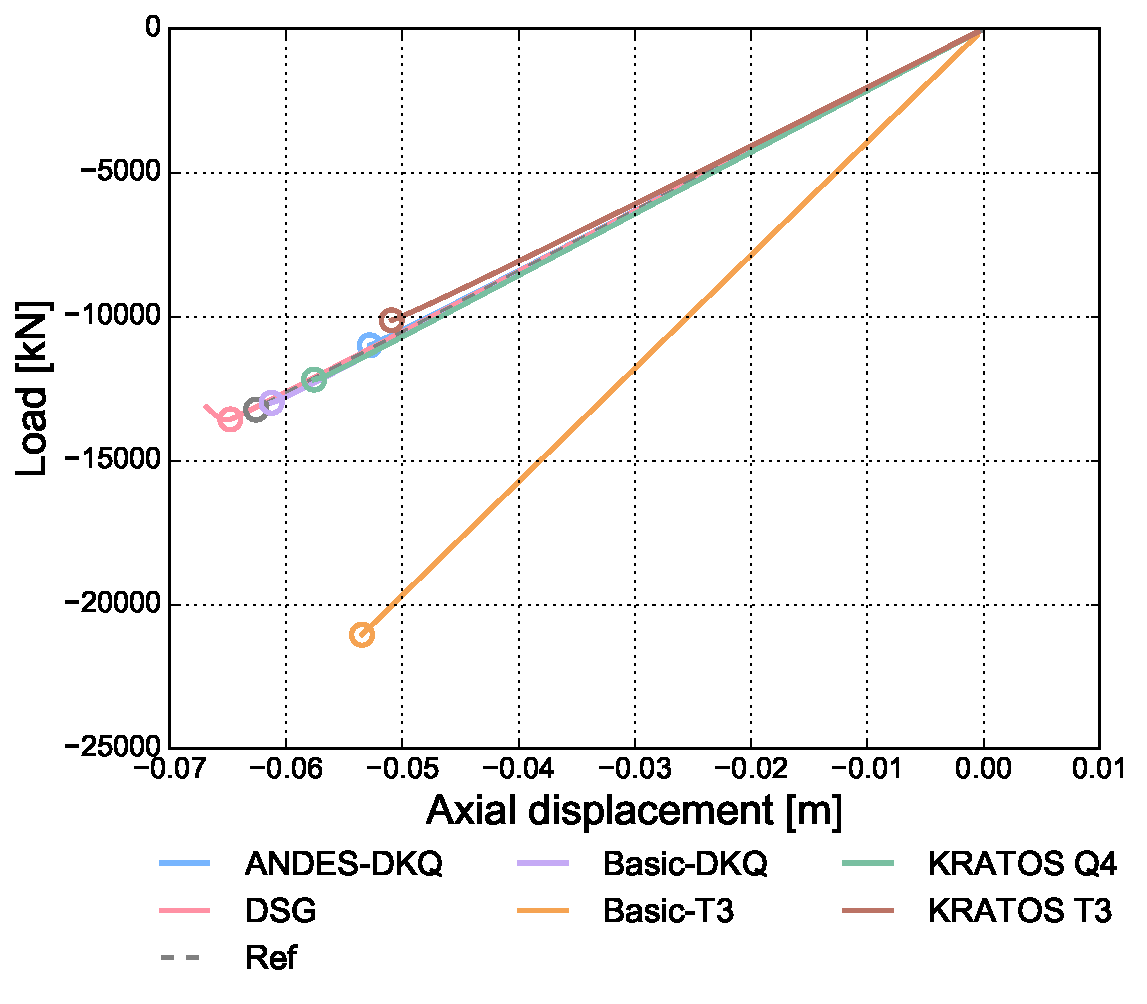
\includegraphics[width=12cm]{images/stability_chs_axial_disp.pdf}
	\caption{CHS buckling: axial displacement vs axial load}
	\label{pic:eulerchs1}
\end{figure}

The results above highlight the poor performance of the un-enhanced Basic-T3 element, with it's large over-estimation of the critical load a symptom of severe transverse shear locking. Accordingly, this poor performance also demonstrates the efficacy of the DSG element enhancements with the DSG results aligning quite well with the remaining elements and the reference beam theory solution (which has a first order displacement calculated from an axial stiffness of $EA/L$). The Basic-DKQ element is also quite close to the reference solution most likely because transverse shear locking is mitigated by the DKQ bending formulation while the effect of membrane locking (which this element is susceptible to) is minimized by the fine mesh employed (due to reduced element out of plane warping). Despite this, differences do indeed appear between the Basic-DKQ and ANDES-DKQ elements, the latter of which suggests a lower buckling limit along with the Kratos-T3 thin shell element. To gain more insight into this difference between these two elements and the rest, the axial load is plot against the lateral X-displacement taken at the beam mid-point $(x,y,z) = (D/2,0,L/2)$.

\begin{figure}[H]
	\centering
	\def\svgwidth{\columnwidth}
	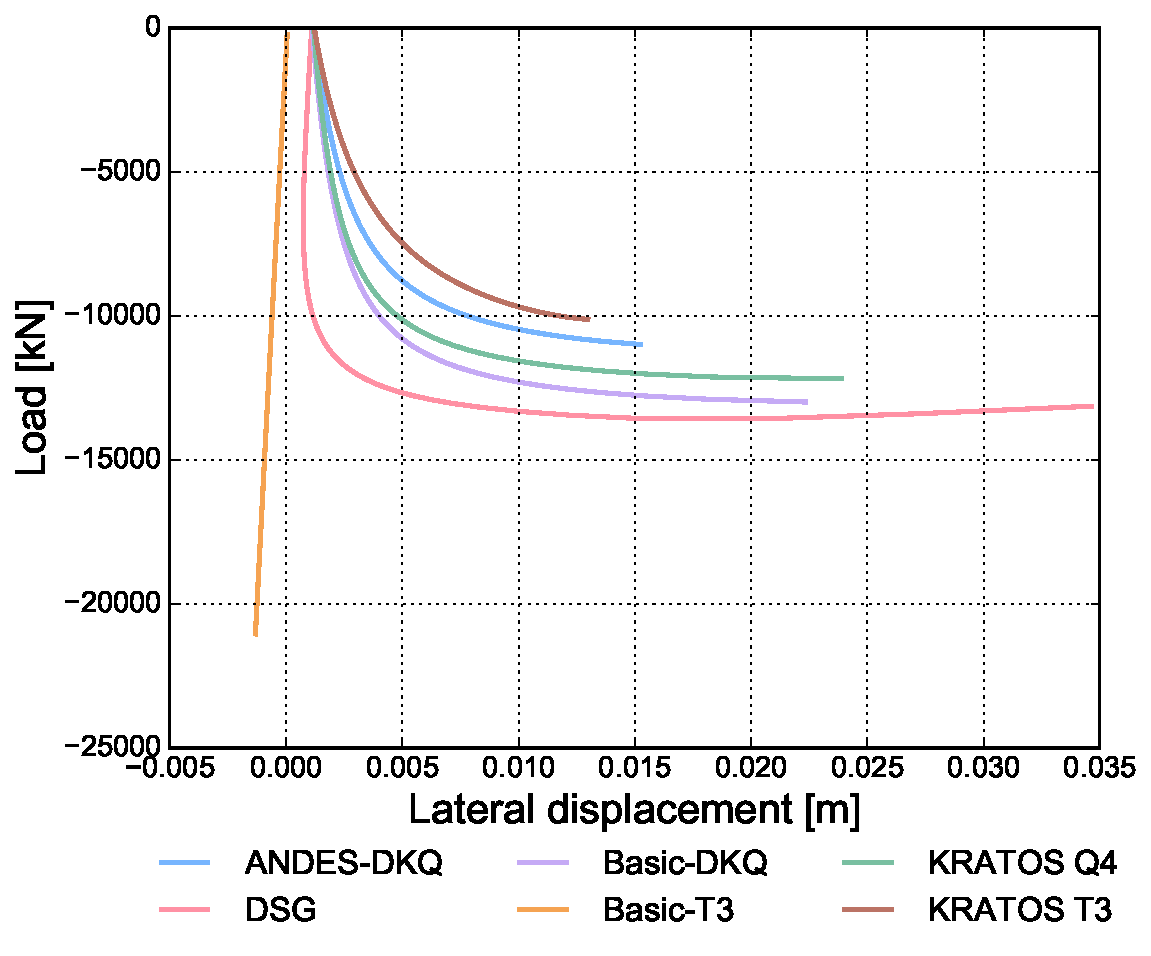
\includegraphics[width=12cm]{images/stability_chs_trans_disp.pdf}
	\caption{CHS buckling: lateral displacement vs axial load}
	\label{pic:eulerchs2}
\end{figure}

The alternative perspective presented above confirms the exceedingly poor performance of the Basic-T3 element once again. As previously identified, the ANDES-DKQ and Kratos-T3 elements predict low buckling loads for the system, however the plot above indicates that these are attached to reduced lateral displacements too (compared to the Kratos-Q4, Basic-DKQ and DSG elements). Clearly the various reasonable elements are expressing the system behaviour in different ways with the greatest difference occurring between the Kratos-T3 and DSG elements. To gain further insight into the behaviour of these two envelope cases, the following figures show X and Y displacements of the Kratos-T3 and DSG models at the onset of instability plot at 6.7x deformation with the same contour limits.

\begin{figure}[H]
	%\centering
	\subfloat[Kratos-T3 X-displacement]
	{\label{ref_label1}
		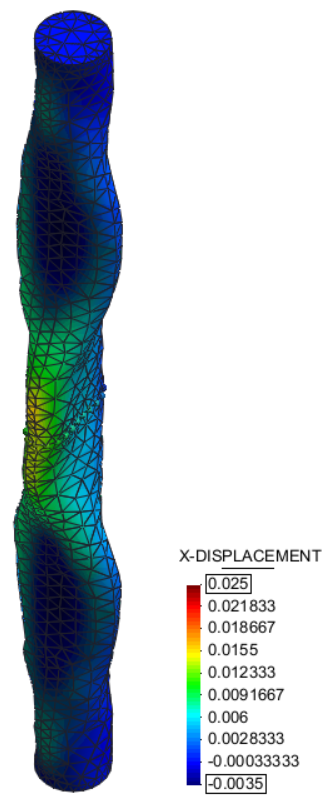
\includegraphics[width=3.5cm]
		{images/chs_kratos_tri_x.png}}
	\subfloat[DSG X-displacement]
	{\label{ref_label1}
		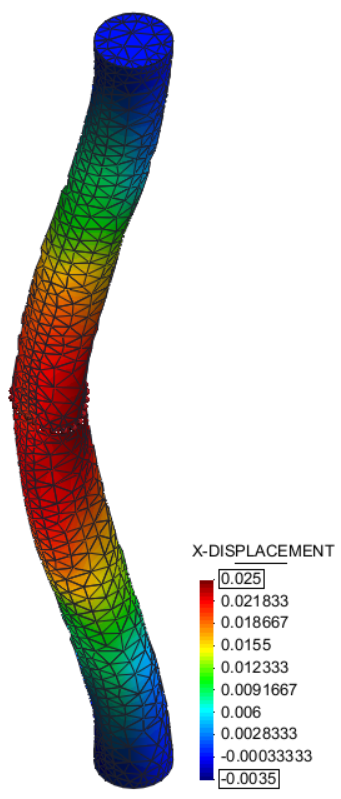
\includegraphics[width=3.5cm]
		{images/chs_dsg_x.png}}
	\subfloat[Kratos-T3 Y-displacement]
	{\label{ref_label2}
		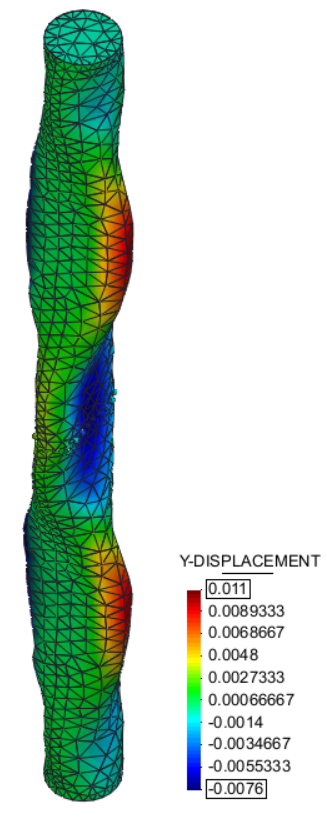
\includegraphics[width=3.5cm]
		{images/chs_kratos_tri_y.png}}
	\subfloat[DSG Y-displacement]
	{\label{ref_label2}
		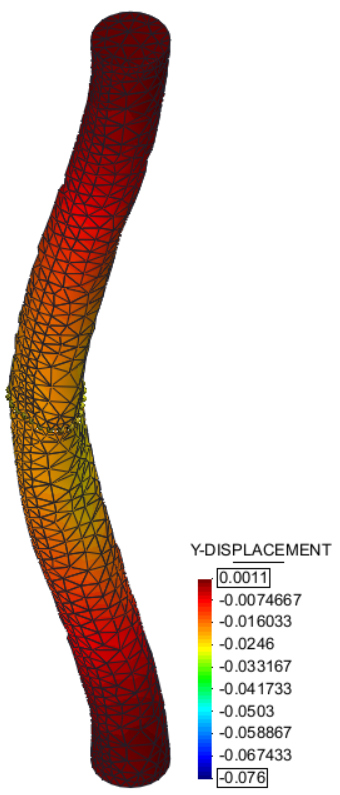
\includegraphics[width=3.5cm]
		{images/chs_dsg_y.png}}
	\caption{\label{chs buckling pics1}CHS buckling: Kratos-T3 and DSG displacement plots at the onset of instability}
\end{figure}

The plots above demonstrate the strikingly different structural behaviours modelled by the two elements using exactly the mesh, boundary conditions and loading conditions. Local ovalisation of the CHS appears to drive buckling in the Kratos-T3 case, whereas the DSG element predominantly maintains the circular cross section throughout and exhibits deformation one would expect from a beam element, explaining the close similarity between the DSG and reference beam results. The differences between the Kratos-T3 (3-parameter) and DSG (5-parameter) elements can be explained by their underlying formulation and the resolving power each posseses. Despite the slenderness ratio $R/t = 20$ of the problem being suitable for both thin and thick shell use, it's intuitive that at this point the 5-parameter model would be more reluctant than the 3-parameter model to predict out of plane bending behaviour, leading to ovalisation. Furthermore, the DSG element is computed with a single Gauss Point while the Kratos-T3 element is computed with 3 Gauss Points which confers a relative advantage in resolving complex local displacement fields (such as local ovalisation).

For completeness, the X and Y displacements of the ANDES-DKQ and Basic-DKQ models at the onset of instability are also plotted below with 6.7x deformation and equilibrated contour limits.

\begin{figure}[H]
	%\centering
	\subfloat[ANDES-DKQ X-displacement]
	{\label{ref_label1}
		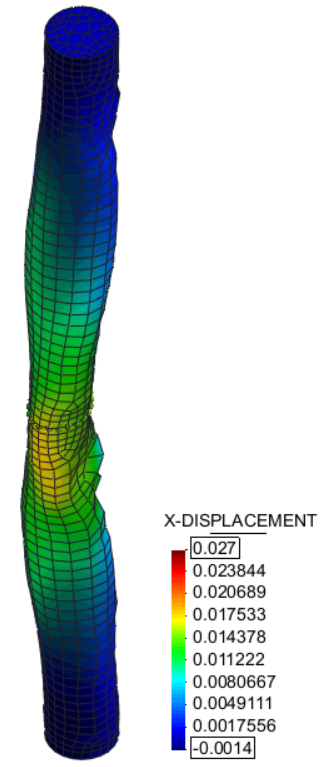
\includegraphics[width=3.5cm]
		{images/chs_thin_quad_x.png}}
	\subfloat[Basic-DKQ X-displacement]
	{\label{ref_label1}
		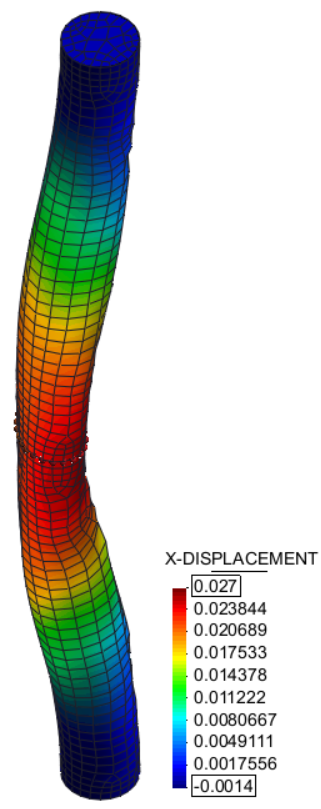
\includegraphics[width=3.5cm]
		{images/chs_thin_quad_basic_x.png}}
	\subfloat[ANDES-DKQ Y-displacement]
{\label{ref_label1}
	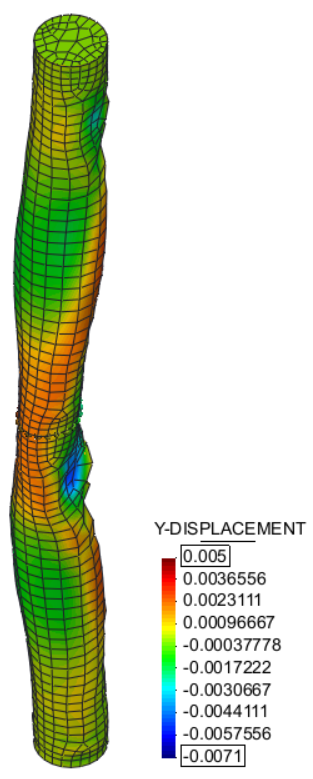
\includegraphics[width=3.5cm]
	{images/chs_thin_quad_y.png}}
\subfloat[Basic-DKQ Y-displacement]
{\label{ref_label1}
	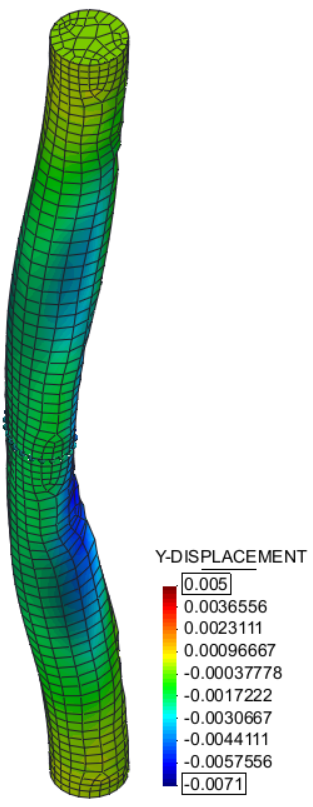
\includegraphics[width=3.5cm]
	{images/chs_thin_quad_basic_y.png}}
	\caption{\label{chs buckling pics2}CHS buckling: ANDES-DKQ and Basic-DKQ displacement plots at the onset of instability}
\end{figure}

In this comparison, the differences in deformation behaviour is solely due to the ANDES enhancement that mitigates membrane locking. An unstructured quadrilateral mesh of a curved surface, such as above, is a quintessential situation for membrane locking to arise. It can be seen that the ANDES-DKQ case exhibits ovalisation of the cross section as expected by it's similarity to the aforementioned Kratos-T3 results. Contrasting this, the Basic-DKQ results display an incredibly minor amount of ovalisation, reduced from it's enhanced counterpart solely due to unmitigated membrane locking, with a more classical beam deflection shape maintaining a relatively constant cross section throughout. Although the ANDES-DKQ and the Basic-DKQ have the same local displacement field resolving power of 4 Gauss Points and also have 3-parameter based enhanced bending formulations, the membrane formulation leading to the prevention or inclusion of membrane locking is the decisive factor here and evidently has a significant impact on the results obtained.

Through the comparison of results obtained with various elements employing different element enhancements it is clear that structural modelling with shells, as discussed in section \ref{Structural modelling with shells}, requires careful consideration of simplifications and assumptions made. For the analysed problem of a CHS beam buckling dimensional reduction can be reasonably varied between a 1D and 2D approach, as explored. Undertaking a one dimensional beam approach may yield quick and acceptable 'ballpark' results, such as Euler's buckling formula, but it also immensely filters the space of possible mechanical expressions resolvable, such as local ovalisation which was seen to form an important driver in some of the results obtained. However, simply adopting a two dimensional shell approach to the problem did not homogenize all results, as was seen. Element base formulations, element enhancements, element order and mesh were all important factors strongly affecting results and correspond to questions that must be answered upon entering the shell regime. 

\subsection{Shear wrinkling of thin membrane}

asdafdf

\begin{figure}[H]
	\centering
	\def\svgwidth{\columnwidth}
	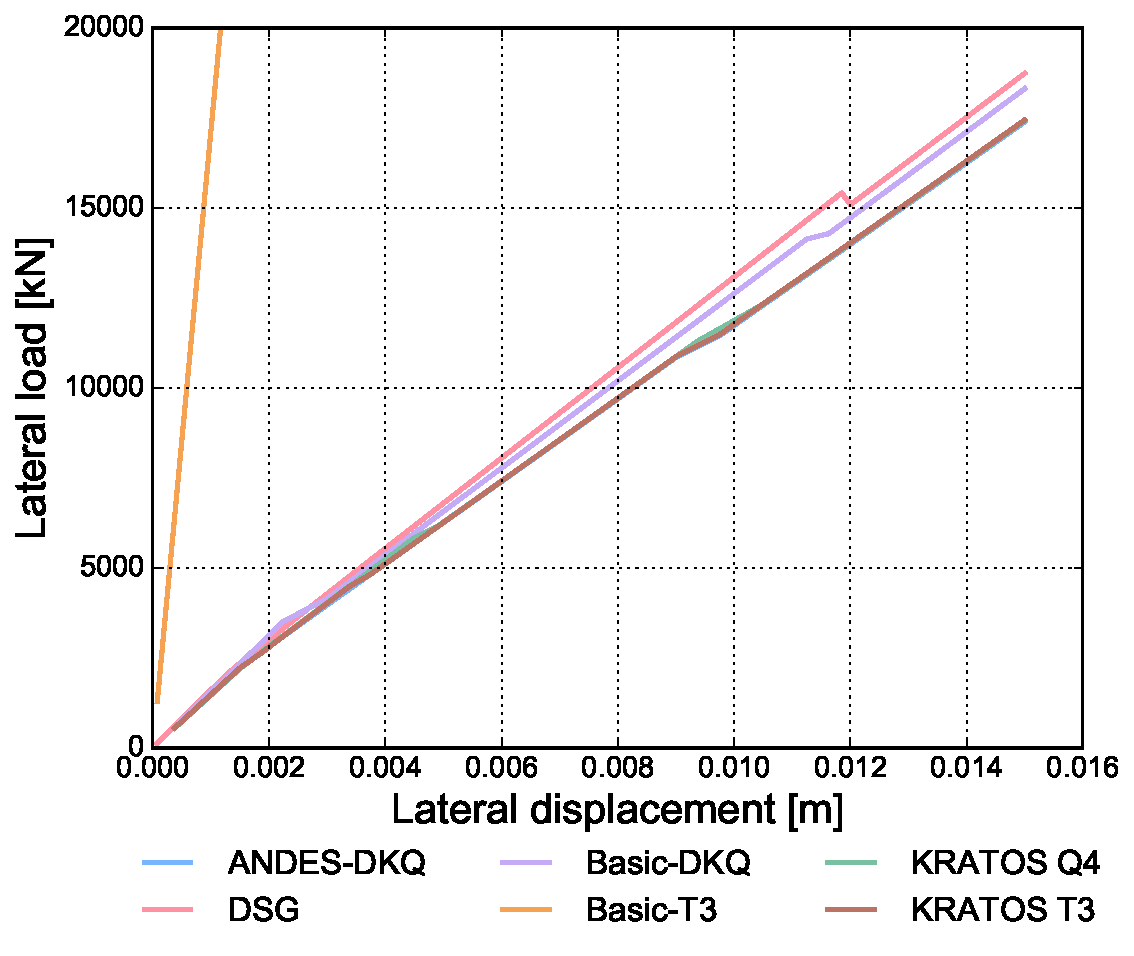
\includegraphics[width=12cm]{images/stability_wrinkle_axial_disp.pdf}
	\caption{Plate shear stability analysis: lateral displacement vs lateral load}
	\label{pic:wrinkle1}
\end{figure}

asdfadsf

\begin{figure}[H]
	\centering
	\def\svgwidth{\columnwidth}
	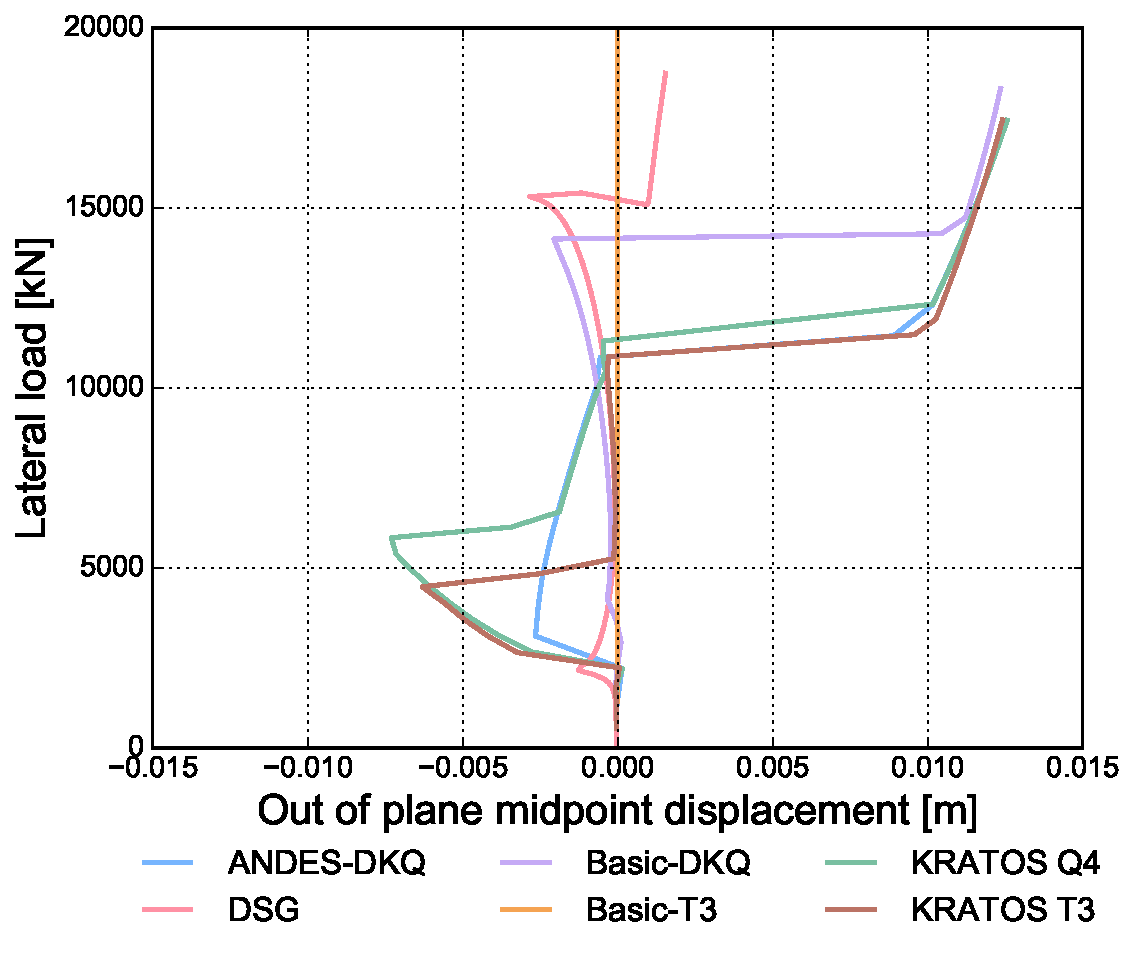
\includegraphics[width=12cm]{images/stability_wrinkle_pointtrans_disp.pdf}
	\caption{Plate shear stability analysis: out of plane mid-point displacement vs lateral load}
	\label{pic:wrinkle2}
\end{figure}

asdfadf

\begin{figure}[H]
	\centering
	\def\svgwidth{\columnwidth}
	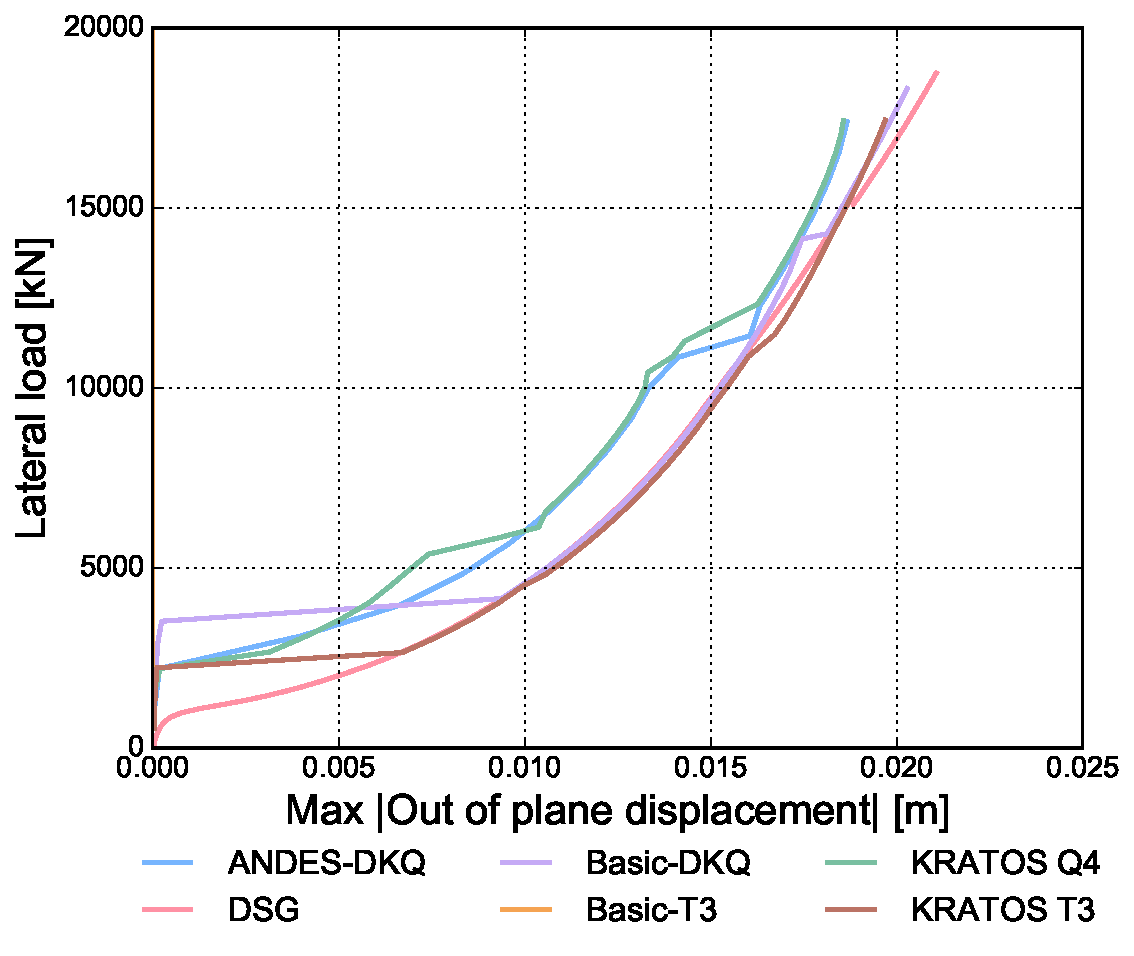
\includegraphics[width=12cm]{images/stability_wrinkle_abstrans_disp.pdf}
	\caption{Plate shear stability analysis: maximum absolute out of plane displacement vs lateral load}
	\label{pic:wrinkle3}
\end{figure}

asdfadsf
